% !TEX TS-program = pdflatex
% !TEX encoding = UTF-8 Unicode

% This is a simple template for a LaTeX document using the "article" class.
% See "book", "report", "letter" for other types of document.

\documentclass[11pt]{article} % use larger type; default would be 10pt

\usepackage[utf8]{inputenc} % set input encoding (not needed with XeLaTeX)

\usepackage{amsfonts}

%%% Examples of Article customizations
% These packages are optional, depending whether you want the features they provide.
% See the LaTeX Companion or other references for full information.

%%% PAGE DIMENSIONS
\usepackage{geometry} % to change the page dimensions
\geometry{a4paper} % or letterpaper (US) or a5paper or....
% \geometry{margin=2in} % for example, change the margins to 2 inches all round
% \geometry{landscape} % set up the page for landscape
%   read geometry.pdf for detailed page layout information

\usepackage{graphicx} % support the \includegraphics command and options

% \usepackage[parfill]{parskip} % Activate to begin paragraphs with an empty line rather than an indent
\usepackage{parskip}
%%% PACKAGES
\usepackage{booktabs} % for much better looking tables
\usepackage{array} % for better arrays (eg matrices) in maths
\usepackage{paralist} % very flexible & customisable lists (eg. enumerate/itemize, etc.)
\usepackage{verbatim} % adds environment for commenting out blocks of text & for better verbatim
\usepackage{subfig} % make it possible to include more than one captioned figure/table in a single float
% These packages are all incorporated in the memoir class to one degree or another...

%%% HEADERS & FOOTERS
\usepackage{fancyhdr} % This should be set AFTER setting up the page geometry
\pagestyle{fancy} % options: empty , plain , fancy
\renewcommand{\headrulewidth}{0pt} % customise the layout...
\lhead{}\chead{}\rhead{}
\lfoot{}\cfoot{\thepage}\rfoot{}

%%% SECTION TITLE APPEARANCE
\usepackage{sectsty}
\allsectionsfont{\sffamily\mdseries\upshape} % (See the fntguide.pdf for font help)
% (This matches ConTeXt defaults)

%%% ToC (table of contents) APPEARANCE
\usepackage[nottoc,notlof,notlot]{tocbibind} % Put the bibliography in the ToC
\usepackage[titles,subfigure]{tocloft} % Alter the style of the Table of Contents
\renewcommand{\cftsecfont}{\rmfamily\mdseries\upshape}
\renewcommand{\cftsecpagefont}{\rmfamily\mdseries\upshape} % No bold!

%%% END Article customizations

%%% The "real" document content comes below...

\title{Analysis I: Übung 7}
\author{Michel Heusser}
%\date{} % Activate to display a given date or no date (if empty),
         % otherwise the current date is printed 

\begin{document}
\maketitle

\section{Theorie}

\subsection{Kurvendiskussion}

\underline{Definition:} $x_0$ ist eine {\bf lokale Extremalstelle} von $f: A \in \mathbb{R} \rightarrow B \in \mathbb{R}$, $x \rightarrow f(x)$ falls es gilt:
\begin{itemize}
\item Formal: $\exists \epsilon>0: f(x) \leq f(x_0)$ oder $f(x) \geq f(x_0)$ $\qquad \forall x\in (x_0-\epsilon,x_0 + \epsilon)$
\item Formal wörtlich: Es existiert ein auf $x_0$ zentriertes Intervall, so, dass im Intervall alle Funktionswerte kleiner als $f(x_0)$ oder alle Funktionswerte grösser als $f(x_0)$ sind.
\end{itemize}

$Bemerkung:$ Wenn $x_0$ eine lokale Extremalstelle ist und es den grössten Funktionswert $f(x_0)$ im Intervall hat, dann ist $x_0$ ein {\bf lokales Maximum}, wenn $x_0$ eine Extremalstelle ist und es den kleinsten Funktionswert im Intervall hat, dann ist sie ein {\bf lokales Minimum}.

\subsubsection{Beispiel}

$f: \mathbb{R} \rightarrow \mathbb{R}$, $x\rightarrow f(x)$

$f(x) := \left \{ 
\begin{array}{l  l}
	-x & x<0\\
	2x+5 & 0\leq x\leq 1\\
	\ln(x) & x > 1
\end{array} \right.$ \\

Ist $x_0=1$ eine lokale Extremalstelle? 

Ja. Durch graphische Darstellung stellt man fest, dass es ein $\epsilon$ existiert (z.B. $\epsilon = 1$), so, dass $f(x_0) = 7 \geq f(x)$ für alle $x$ im intervall $(x_0 - \epsilon, x_0 + \epsilon) = (0,2)$. $x_0$ ist Ferner ein lokales Maximum

\subsubsection{Beispiel}
$f: [-3,5] \rightarrow \mathbb{R}$, $x\rightarrow f(x) := |x|$

Ist $x_0 = 5$ eine lokale Maximalstelle?
\\\\
Nein. Es existiert kein $(x_0 - \epsilon, x_0 + \epsilon)$ mit $\epsilon >0$, so, dass $f(x_0) \geq f(x)$ (oder $f(x_0) \leq f(x))$ für alle $x$ im Intervall, weil $f(x)$ gar nicht definiert ist auf der Rechten seite von $x_0=5$ \\

\underline{Definition:} $x_0$ ist eine {\bf globale Extremalstelle} von $f: A \in \mathbb{R} \rightarrow B \in \mathbb{R}$, $x \rightarrow f(x)$ falls es gilt:
\begin{itemize}
\item Formal: $f(x_0) \leq f(x)$ oder $f(x_0) \geq f(x) \qquad \forall x \in D(f)$
\item Formal wörtlich: $f(x_0)$ ist das grösste/kleinste Funktionswert der ganzen Funktion.
\end{itemize}

$Bemerkung:$ Wenn $x_0$ eine globale Extremalstelle ist und es den grössten Funktionswert $f(x_0)$ der Funktion, dann ist $x_0$ ein {\bf globales Maximum}, wenn $x_0$ eine globale Extremalstelle ist und es den kleinsten Funktionswert der Funktion hat, dann ist sie ein {\bf lokales Minimum}.


\subsubsection{Beispiel}

$f: [-1,1] \rightarrow \mathbb{R}$, $x\rightarrow f(x)$

$f(x) := \left \{ 
\begin{array}{l  l}
	-x & x<0\\
	5 & x=0\\
	x & x > 0
\end{array} \right.$ \\

Ist $x_0 = 0$ eine globale Extremalstelle?

Ja. Ein globales Maximum

\subsubsection{Beispiel}

$f: [-2,2] \rightarrow \mathbb{R}$, $x\rightarrow f(x)$

$f(x) := \left \{ 
\begin{array}{l  l}
	x & -2\leq x\leq0\\
	-x^2 & 0< x \leq 2\\
	\end{array} \right.$ \\

Ist $x_0=2$ eine lokale Extremalstelle?

Nein. Aber schon ein globales Minimum


\subsubsection{Beispiel}

$f: [-1,1] \rightarrow \mathbb{R}$, $x\rightarrow f(x) = x^2-x^4+5$
 
Ist $x_0 = 0$ eine globale Extremalstelle?
\\\\
Ja, ein globales (und lokales) Maximum\\\\

\underline{Satz}: Für $f: A \in \mathbb{R} \rightarrow B \in \mathbb{R}$, $x \rightarrow f(x)$ und $x_0\in D(f)$ gilt:
\begin{itemize}
\item $f$ ist in $x_0$ {\bf differenzierbar} und $x_0$ ist eine {\bf lokale Extremalstelle} \\ $\Rightarrow f'(x_0) = 0$
\end{itemize}

\subsubsection{Beispiel}

$f: [-1,1] \rightarrow \mathbb{R}$, $x\rightarrow f(x) = x^2-x^4+5$

Hier ist $f$ bei $x_0 = 0$ differenzierbar und $x_0$ ist eine lokale Extremalstelle $\Rightarrow f'(x_0) = 0$\\

Nachweis: $f'(x_0) = 2x_0 - 4x_0^3 = 0$

\subsubsection{Beispiel}

Obwohl für $f: A \in \mathbb{R} \rightarrow B \in \mathbb{R}$, $x \rightarrow f(x) = (x-3)^3 + 5$,\\ $f'(x_0=3) = 0$ ist, heisst es nicht, dass $x_0$ eine lokale Extremalstelle ist (und es ist Tatsächlich keine!), weil eben nur "$\Rightarrow$" und \emph{nicht} "$\Leftarrow$" gilt.\\

\underline{Satz}: Für $f: A \in \mathbb{R} \rightarrow B \in \mathbb{R}$, $x \rightarrow f(x)$ und $f$ differenzierbar in $x_0\in D(f)$ gilt:
\begin{enumerate}
\item ($f'(x_0) = 0 $ und $f'(x)$ wechselt sein Vorzeichen in $x_0) \Rightarrow (x_0$ ist eine lokale Extremalstelle)
\\\emph{Bemerkung:} Wenn der Vorwechsel von + auf - ist, ist $x_0$ eine lokale Maximalstelle, umgekehrt eine lokale Minimalstelle (natürlich wenn $x$ von der linken Seite von $x_0$ auf der rechten Seite sich bewegt)
\item ($f'(x_0)=0$ und $f''(x_0) \neq 0$ ($f$ muss 2 mal diff'bar sein!))$\Rightarrow (x_0$ ist eine lokale Extremalstelle). \\\emph{Bemerkung:} Hier gilt dann: $f''(x_0) >0 \Rightarrow$ $x_0$ lokales Minimum und $f''(x_0) < 0 \Rightarrow$ $x_0$ lokales Maximum! Falls $f'(x_0) = 0$ und $f''(x_0) = 0$ (also, die linke Seite von 2. gilt nicht), dann Kriterium 1. benutzen, es könnte schon sein dass $x_0$ eine lokale Extremalstelle ist!

\end{enumerate}

 \subsubsection{Beispiel}

$f: [-2,\frac{\pi}{2}] \rightarrow \mathbb{R}$, $x\rightarrow f(x)$

$f(x) := \left \{ 
\begin{array}{l  l}
	-x^2+4 & -2\leq x\leq0\\
	4\cos(x) & 0 <x \leq \frac{\pi}{2}\\
	\end{array} \right.$ \\


Wir suchen globale Extremalstellen von $f$:\\

Man kann zeigen (oder sich graphisch überlegen), dass $f$ differenzierbar ist. Wir suchen erst Stellen $x_0$ wo $f'(x_0) = 0$. Dann überprüfen wir ob es ein Vorzeigenwechsel in $x_0$ statt findet.

$f'(x_0) = 0 \Rightarrow x_0 = 0$

Wegen: $ f'(x) = \left \{ 
\begin{array}{l  l}
	-2x & -2\leq x\leq0\\
	-4\sin(x) & 0 <x \leq \frac{\pi}{2}\\
	\end{array} \right.$ \\

Wir stellen klar fest, dass bei $x_0$ ein Vorzeichenwechsel statt findet! Deswegen ist $x_0$ eine lokale Extremalstelle. (Hier ist die Funktion in $x_0$ nicht zweimal Differenzierbar, und deswegen kann man die zweite Ableitung nicht benutzen!)

\subsubsection{Beispiel}
$f: \mathbb{R} \rightarrow \mathbb{R}$, $x\rightarrow f(x)$

$f(x) := x^3+ 4x^2$

$f$ ist zweimal Differenzierbar. Mit $f'(x_0) = 0$ suchen wir mögliche Extremalstellen. Daraus bekommen wir $x_{0,1} = 0$ und $x_{0,2} = -\frac{8}{3}$. Da $f''(x_{0,1})=8>0$ und $f''(x_{0,2}=-8)<0$ folgt, dass $x_{0,1}$ eine lokale Minimalstelle ist und $x_{0,2}$ eine lokale Maximalstelle ist.

\underline{Definition:} $x_0$ ist eine {\bf Wendestelle} von der (in $x_0$) zweimal differenzierbaren Funktion $f: A \in \mathbb{R} \rightarrow B \in \mathbb{R}$, $x \rightarrow f(x)$ falls $f$ seine Krümmung in $x_0$ die Richtung ändert (linksgekrümmt  $\rightarrow$ rechtsgekrümmt oder umgekehrt).\\

\subsubsection{Beispiel}

$f: [-\frac{\pi}{2},\frac{\pi}{2}] \rightarrow \mathbb{R}$, $x\rightarrow f(x) := \sin(x)$

Wir sehen, dass $f$ im Intervall $[-\frac{\pi}{2}, 0)$ rechtsgekrümmt ist und im Intervall $(0,\frac{\pi}{2}]$ sie Linksgekrümmt ist (in $x_0=0$ ist sie gar nicht gekrümmt). Aus der Symmetrie der Funktion, wissen wir, dass die Funktion in der Symmetriestelle $x_0=0$ ihre Krümmung wechseln musste $\Rightarrow$ $x_0$ ist eine Wendestelle!

\underline{Satz:} für eine in $x_0$ zweimal differenzierbare Funktion $f: A \in \mathbb{R} \rightarrow B \in \mathbb{R}$, $x \rightarrow f(x)$ gilt:
\begin{enumerate}
\item $x_0$ ist eine Wendestelle $\Rightarrow$ $f''(x_0) = 0$\qquad (Umgekehrt aber nicht unbedingt!)
\item $f''(x_0) > 0 \Rightarrow f$ in $x_0$ linksgekrümmt
\item  $f''(x_0) < 0 \Rightarrow f$ in $x_0$ rechtsgekrümmt
\item $f''$ hat in $x_0$ einen Vorzeichenwechsel $\Rightarrow$ $x_0$ ist eine Wendestelle (ist mit 2. und 3. dann konsistent mit Definition einer Wendestelle!)
\item ($f''(x_0)=0$ und $f'''(x_0) \neq 0) \Rightarrow$ ($x_0$ ist eine Wendestelle) \\
\emph{Bemerkung:} Dieser Punkt ist eine andere Überprüfung von 4., weil es setzt voraus, dass $f$ wirklich die Richtung der Krümmung wechselt und nicht nur auf keine Krümmung geht und dann zurrück in die ursprüngliche Krümmung geht (siehe Beispiel). Falls die linke Seite von Kriterium 5 nicht gilt ($f''(x_0)=0$ und $f'''(x_0)=0$) muss man Kriterium 4. benutzen, es könnte schon sein, dass $x_0$ eine Wendestelle ist!.
\end{enumerate}


\subsubsection{Beispiel}

$f: [-4,2] \rightarrow \mathbb{R}$, $x\rightarrow f(x) = x^3+4x^2$
 
Wir suchen Wendestellen:

Wir benutzen $f''(x_0)= 6x_0 + 8 =0$ und wir bekommen $x_0= -\frac{4}{3}$ als mögliche Wendestelle. Wir müssen, dann überprüfen, dass $x_0$ wirklich eine Wendestelle ist. Entweder mit Punkt 4. oder 5. vom obigen Satz. \\

\underline{Punkt 4.}:  Es ist leicht zu überprüfen, dass $f''(x) = 6x+8$ links von $x_0= -\frac{4}{3}$ negativ ist und rechts davon positiv $\Rightarrow$ $x_0$ ist eine Wendestelle

\underline{Punkt 5}: $f'''(x_0) = 6 \neq 0$ $\Rightarrow$ $x_0$ ist eine Wendestelle!

\section{Tipps}


\subsection{Online-Teil}
Immer zurrück auf die Definition (Handouts):
Für hyperbolische Funktionen:

$\sinh(x):= \frac{1}{2}(e^x - e^{-x})$\\
$\cosh(x):= \frac{1}{2}(e^x + e^{-x})$\\
$\tanh(x) : = \frac{\sinh(x)}{\cosh{x}}$
\subsection{Aufgabe 2}
Globale Extremalstellen (Maximas und Minimas) finden einer Funktion:
\begin{enumerate}
\item $f'(x_0) = 0 \Rightarrow x_0$ (mögliche lokale Extremalstellen auftellen)
\item Überprüfen, dass sie wirklich lokale Extremalstellen sind.
\item Funktionswerte von Extremalstellen aufstellen (Kandidaten für globale Extremalstellen aufstellen)
\item Falls vorhanden, Funktionswerte der Rände anschauen (Kandidaten für globale Extremalstellen aufstellen)
\item Entscheiden welche Kandidaten (für globale Extremalstellen) die eigentliche globale Extremalstellen ist (falls es mehrere gibt)
\end{enumerate}

Hier muss man Aufpassen weil es undendlich viele Extremalstellen gibt!
\subsection{Aufgabe 3}

Das einzige Gebebene ist der Radius $r$ der Kugel. Skizze (2D) aufstellen und $\alpha$ (Öffnungswinkel der Kegel) als gegeben Annehmen). Durch Trigonometrische beziehungen die restlichen Grössen bestimmen und Volumen des Kegels (in abhängigkeit von $\alpha$ aufstellen), also $V(\alpha)=\frac{1}{3} \pi R^2(\alpha) h(\alpha)$. Minimum von $V(\alpha)$ bestimmen! 

\subsection{Aufgabe 4}
In dieser Aufgabe, muss man die tiefste Höhe finden, die vom Punkt $S$ überhaupt erreicht werden kann. Nach Figure \ref{fig:a4} kann man alle geometrische relevante Daten in abhängigkeit des Winkels $\alpha$ bestimmen. \\
\begin{figure}[H]
\centering
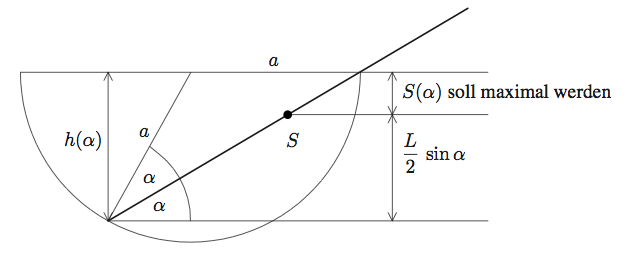
\includegraphics[width=0.7\textwidth]{uebung7A4.png}
\caption{Skizze zur Aufgabe 4}
\label{fig:a4}
\end{figure}

Die funktion $S(\alpha)$ muss also maximiert werden (da liegt $S$ am tiefsten). Man muss erstmal den Definitionsbereich $D(S)$ bestimmen indem man die erlaubten $\alpha$-Werten ermittelt. Folglich sucht man die lokale Maximalstellen, untersucht man die Rände und man stellt die Kandidaten für das globale Maximum auf. Nach dem Vergleich von Funktionswerten entscheidet man sich für die globale Maximalstelle mit ihrem entsprechenden Maximalwert.  



\end{document}



